\documentclass[twoside]{article}
\usepackage{mdframed}
\usepackage[hmarginratio=1:1,top=32mm,columnsep=20pt]{geometry} % Document margins
\usepackage{multicol} % Used for the two-column layout of the document
\usepackage[hang, small,labelfont=bf,up,textfont=it,up]{caption} % Custom captions under/above floats in tables or figures
\usepackage{booktabs} % Horizontal rules in tables
\usepackage{float} % Required for tables and figures in the multi-column environment - they need to be placed in specific locations with the [H] (e.g. \begin{table}[H])
\usepackage{hyperref} % For hyperlinks in the PDF
\usepackage{amsmath,amsthm,amssymb}
\usepackage{lettrine} % The lettrine is the first enlarged letter at the beginning of the text
\usepackage{paralist} % Used for the compactitem environment which makes bullet points with less space between them
\usepackage{tikz}
\usepackage{esint}
\usepackage{centernot}
\usepackage{lmodern}
\usetikzlibrary{3d}
\usetikzlibrary{patterns,calc,hobby}
\usetikzlibrary{decorations.pathreplacing}
\tikzset{
	partial ellipse/.style args={#1:#2:#3}{
		insert path={+ (#1:#3) arc (#1:#2:#3)}
	}
}
\usepackage{xcolor}

\usepackage{fancyhdr} % Headers and footers
\pagestyle{fancy} % All pages have headers and footers
\fancyhead{} % Blank out the default header
\fancyfoot{} % Blank out the default footer
\fancyhead[C]{Jimmy Yue $\bullet$ Statistics $\bullet$ Jimmy Yue} % Custom header text
\fancyfoot[RO,LE]{\thepage} % Custom footer text

\newmdenv[skipabove=7pt,
rightline=false,
leftline=true,
topline=false,
bottomline=false,
skipbelow=5pt,
linecolor=black,
innerleftmargin=5pt,
innerrightmargin=5pt,
innertopmargin=5pt,
leftmargin=0cm,
rightmargin=0cm,
linewidth=4pt,
innerbottommargin=5pt]{cBox}

\theoremstyle{definition}
\newtheorem*{solutionT}{Solution}

\newenvironment{solution}{\begin{cBox}\begin{solutionT}}{\hfill{\scriptsize\ensuremath{\square}}\end{solutionT}\end{cBox}}

%%%%%%%%%%%%%%%%%%%%%%%%%%%%%%%%%%%%%%%%%%%%%%%%%%%%%%%%%%%%%%%%%%%%%%%%%%%%%%%%%%%%%%%%%%%%
\newcommand{\vect}[1]{\vec{\pmb{#1}}}
\newcommand{\uvect}[1]{\hat{\mathbf{#1}}}
\newcommand{\leviciv}{\epsilon_{ijk}}

\newmdenv[skipabove=7pt,
rightline=false,
leftline=true,
topline=false,
bottomline=false,
skipbelow=5pt,
linecolor=black,
innerleftmargin=5pt,
innerrightmargin=5pt,
innertopmargin=5pt,
leftmargin=0cm,
rightmargin=0cm,
linewidth=4pt,
innerbottommargin=7,
backgroundcolor=light-gray]{dBox}



\theoremstyle{definition}
\newtheorem*{proof1}{Definition}

\newenvironment{ddef}{\begin{dBox}\begin{proof1}}{\hfill{\scriptsize}\end{proof1}\end{dBox}}
\newcommand{\pdif}[2]{\frac{\partial#1}{\partial#2}}
\definecolor{light-gray}{gray}{0.85}
%----------------------------------------------------------------------------------------
%-	TITLE SECTION
%----------------------------------------------------------------------------------------

\title{\vspace{-15mm}\fontsize{24pt}{10pt}\selectfont\textbf{Statistics - Week 1}} % Article title

\author{
\large
\textsc{Jimmy Tsz Ming Yue}\thanks{440159151}\\[2mm] % Your name
\normalsize University of Sydney \\ % Your institution
\normalsize \href{mailto:jyue6728@uni.sydney.edu.au}{jyue6728@uni.sydney.edu.au} % Your email address
\vspace{-5mm}
}
\date{}

%----------------------------------------------------------------------------------------

\usepackage{Sweave}
\begin{document}
\Sconcordance{concordance:week1.tex:week1.Rnw:%
1 98 1 1 0 16 1 6 0 1 5 1 2 4 0 2 2 4 0 1 2 1 1 1 2 4 0 1 2 3 1 1 2 7 0 %
2 2 4 0 2 2 4 0 1 2 1 1 1 2 8 0 2 1 9 0 1 2 3 1 1 2 1 0 1 1 5 0 2 1 6 0 %
2 2 7 0 2 2 1 0 1 1 6 0 2 2 1 0 1 1 5 0 2 1 6 0 1 2 3 1 1 2 4 0 1 2 1 1 %
1 2 1 0 1 1 11 0 2 2 6 0 1 2 6 0 1 2 6 0 1 2 8 0 1 2 12 0 1 3 79 1 1 2 %
1 0 1 2 1 0 1 2 1 0 2 1 180 0 2 2 4 0 1 2 7 1 1 2 1 0 1 1 11 0 1 1 5 0 %
1 4 1 0 1 1 4 0 1 3 4 0 1 2 5 1 1 2 1 0 1 3 2 0 1 1 1 2 1 0 1 1 9 0 1 2 %
4 1 1 2 1 0 1 1 1 4 8 0 1 4 1 0 1 5 8 0 1 3 1 0 1 5 8 0 1 2 3 1 1 2 1 0 %
1 1 24 0 1 1 4 0 1 2 4 1}


\maketitle % Insert title

\thispagestyle{fancy} % All pages have headers and footers
\hrule \smallskip

\noindent Semester 2 \quad Statistics \hspace{10.5
cm} 2018
\smallskip
\hrule
\smallskip
\tableofcontents
\section{Importing Files and Important Functions}
To do analysis of files, we first need to import into a the R program. We can use use the code:
\begin{Schunk}
\begin{Sinput}
> #read.delim()
> #scan 
> #read.table
\end{Sinput}
\end{Schunk}
We can find help on any function in R by placing a ? mark in front of a command: for example 
\begin{Schunk}
\begin{Sinput}
> ?read.table()
\end{Sinput}
\end{Schunk}
This is equivalent to the help function:
\begin{Schunk}
\begin{Sinput}
> help("read.table")
\end{Sinput}
\end{Schunk}

We can save a workspace in R using the function:
\begin{Schunk}
\begin{Sinput}
> save.image()
\end{Sinput}
\end{Schunk}
which saves parameters and command history.

\subsection{Basics: Directories}
To get the current working directory:
\begin{Schunk}
\begin{Sinput}
> getwd()
\end{Sinput}
\begin{Soutput}
[1] "/home/jyue/Documents/MDS/STAT/Data_w1"
\end{Soutput}
\end{Schunk}
Furthermore we can change directory using the setwd() command:
\begin{Schunk}
\begin{Sinput}
> setwd("/home/jyue/Documents/MDS/STAT/Data_w1/")
\end{Sinput}
\end{Schunk}
We  can also save image with a specific name as:
\begin{Schunk}
\begin{Sinput}
> save.image("week1.Rdata")
\end{Sinput}
\end{Schunk}
\subsection{Search paths and packages}
In R there exists a base package, which exsists with an installation enviroment of R. There also exists community built "contributed" packages which are available for installation. The search funcction gives a list of attached backages and R objects. 
\begin{Schunk}
\begin{Sinput}
> search()
\end{Sinput}
\begin{Soutput}
[1] ".GlobalEnv"        "package:stats"     "package:graphics" 
[4] "package:grDevices" "package:utils"     "package:datasets" 
[7] "package:methods"   "Autoloads"         "package:base"     
\end{Soutput}
\begin{Sinput}
> library(cluster)
> search()
\end{Sinput}
\begin{Soutput}
 [1] ".GlobalEnv"        "package:cluster"   "package:stats"    
 [4] "package:graphics"  "package:grDevices" "package:utils"    
 [7] "package:datasets"  "package:methods"   "Autoloads"        
[10] "package:base"     
\end{Soutput}
\end{Schunk}
as we can see we have that the third entry of the search function is the cluster library that we have loaded.
\section{Basic elements in R}
\subsection{Concatenate and is.datatype}
Normally in R we work with vectors or Matricies in R. (Another one is a list but that shall be in later sections) The simplest data structure is a numeric vector, which is a singular entity consisting of an ordered collection of numbers. To generate a vector we use the concatenate function:
\begin{Schunk}
\begin{Sinput}
> x = c(10.4, 5.6, 3.1, 6.4, 21.7)
> x
\end{Sinput}
\begin{Soutput}
[1] 10.4  5.6  3.1  6.4 21.7
\end{Soutput}
\begin{Sinput}
> x <- c(10.4, 5.6, 3.1, 6.4, 21.7)
> x
\end{Sinput}
\begin{Soutput}
[1] 10.4  5.6  3.1  6.4 21.7
\end{Soutput}
\end{Schunk}
which are numeric vectors. We can verify that it is numeric through the is.numeric() function:
\begin{Schunk}
\begin{Sinput}
> is.numeric(x)
\end{Sinput}
\begin{Soutput}
[1] TRUE
\end{Soutput}
\end{Schunk}
if we have strings included the boolean returned from is.numeric will return false:
\begin{Schunk}
\begin{Sinput}
> x = c(10.4, "5.6", 3.1, 6.4, 21.7)
> is.numeric(x)
\end{Sinput}
\begin{Soutput}
[1] FALSE
\end{Soutput}
\end{Schunk}
similarly we have the is.character command for strings and is.logical for boolean results:
\begin{Schunk}
\begin{Sinput}
> X <- c("a", "b", "c3", "4")
> is.character(X)
\end{Sinput}
\begin{Soutput}
[1] TRUE
\end{Soutput}
\begin{Sinput}
> X <- c(FALSE, FALSE, TRUE, FALSE)
> is.logical(X)
\end{Sinput}
\begin{Soutput}
[1] TRUE
\end{Soutput}
\end{Schunk}
\subsection{Package Installations}
We can install packages using the install.package(packagename)

We load packages using the forementioned libarary function:
\begin{Schunk}
\begin{Sinput}
> library(e1071)
\end{Sinput}
\end{Schunk}
\section{Matrices}
WE can create matrices using the matrix function:
\begin{Schunk}
\begin{Sinput}
> mymatrix <- matrix(1:20,5,4)
> mymatrix
\end{Sinput}
\begin{Soutput}
     [,1] [,2] [,3] [,4]
[1,]    1    6   11   16
[2,]    2    7   12   17
[3,]    3    8   13   18
[4,]    4    9   14   19
[5,]    5   10   15   20
\end{Soutput}
\end{Schunk}
we can find subsets of matrices through indexing:
\begin{Schunk}
\begin{Sinput}
> mymatrix[1,2] 
\end{Sinput}
\begin{Soutput}
[1] 6
\end{Soutput}
\begin{Sinput}
> #first row second column
> mymatrix[1,]
\end{Sinput}
\begin{Soutput}
[1]  1  6 11 16
\end{Soutput}
\begin{Sinput}
> #frist row
> mymatrix[,1]
\end{Sinput}
\begin{Soutput}
[1] 1 2 3 4 5
\end{Soutput}
\begin{Sinput}
> #first column
> mymatrix[1:2,]
\end{Sinput}
\begin{Soutput}
     [,1] [,2] [,3] [,4]
[1,]    1    6   11   16
[2,]    2    7   12   17
\end{Soutput}
\begin{Sinput}
> #first and second column
> mymatrix[c(1,3),]
\end{Sinput}
\begin{Soutput}
     [,1] [,2] [,3] [,4]
[1,]    1    6   11   16
[2,]    3    8   13   18
\end{Soutput}
\begin{Sinput}
> #first and third column
\end{Sinput}
\end{Schunk}
\section{R markdown}
R markdown is shit so we skip this section
\section{Review of Statistical Concepts}
\subsection{Population and Samples}
\begin{ddef}
  Population: The set of data corresponding to the entire collection of units about which information is sought 
\end{ddef}
Examples of populations include: 
\begin{itemize}
\item Blood Presure: blood pressure readings of all people in Australia
\item The number of languages spoken from ALL currently enrolled students in University of Sydney
\end{itemize}
\begin{ddef}
Sample: A subset of population data that are actually collected in the course of a study.
\end{ddef}
Examples of samples include:
\begin{itemize}
\item Blood pressure readings of $1000$ randomly selected people in Australia
\item The number of lanugages spoken from $500$ randomly selected students currently enrolled in University of Sydney
\end{itemize}
In most studies, it is difficult to obtain information about the
whole population. That is why we rely on samples to make
estimates and inferences related to the whole population.
\subsection{Parameters vs Statistics}
A parameter is a number that describes a population
A statistic is a number that describes a sample
We often estsimate parameters thorough looking at statistics. Population parameters are notationally denoted using Greek letters such as $\mu, \sigma$ whereas statistics we use roman letters such as : $x ,s$ or we can put hats on greek letters such as: 
$\hat{\mu}, \hat{\sigma}$
A parameter is a fixed number usually unknown. A statistic is a variable whose value varies from sample to sample
\subsection{Descriptive Statistics}
Many methods are available for summarising data in both nnumeric and graphical form
\subsubsection{Numeric}
For measures of location we use Mean, Mode, Median
For measures of Spread we use: Standard Deviation, Median absolute deviation, IQR (Inter quartile Range)
we can also use Min, Max Quartle, Five num summaries
\subsubsection{Mean}
Consider a sample of data drawn from some population
\begin{equation}
  \{x_1, \dots x_n\}
\end{equation}
Definition of sample mean: The sum of all observations divided by the number of observations. It is written in symbols as:
\begin{equation}
  \bar{x} = \frac{1}{n} \sum_{i=1}^{n} x_i
\end{equation}
Example:
Consider the following data set:
23, 34, 32, 33, 34, 22, 32, 29, 29, 34, 32, 31 \\
Sample mean = $365 / 12 = 30.4$
\subsubsection{Median}
The median of a set of data is a value $\tilde{x}$ such that at least one half of the observations are less than or equal to $\tilde{x}$ and at least one half of the observations are greater than or equal to $\tilde{x}$. 
Definition of Sample median is:
\begin{enumerate}[(a)]
\item The $(n+1)/2$ largest observation if $n$ odd
\item The average of the $n/2$ and the $n/2 + 1$ if $n$ even

\end{enumerate}
\subsubsection{Mode}
The mode is the most frequently occuring value amongst all the observations in a sample
\subsubsection{Mode or Median}
Both the median and the mean are measures of location, but which
is preferable?. \\
For symmetric data, the mean is usually less variable from sample
to sample than the median.\\
For skewed data, the median is a better measure of location.\\
The median does not reacted as much as the mean by outliers. This
property of the median is known as ‘robustness’.
\subsubsection{Range}
The range of a list is the largest value minus the smallest value.
This gives a quick feeling for the overall spread – but is misleading
because it is solely influenced by two most extreme values.
\subsubsection{Graphical}

\section{Tutorial 1}
\begin{enumerate}
\item Download Communities and Crime dataset from \\
\href{(https://archive.ics.uci.edu/ml/datasets/Communities+and+Crime)}{https://archive.ics.uci.edu/ml/datasets/Communities+and+Crime}

\item Read in the data using RStudio
\begin{solution}
We use the read table command to import the data:
\begin{Schunk}
\begin{Sinput}
> data <- read.csv("communities.data", na.strings = "?", header = FALSE)
> #head(data)
> name <- read.table("communities.names", sep = " ", header = FALSE)
> #name[,2]
> df <- data.frame(data)
> colnames(df) <- name[,2]
> head(df)
\end{Sinput}
\begin{Soutput}
  state county community       communityname fold population householdsize
1     8     NA        NA        Lakewoodcity    1       0.19          0.33
2    53     NA        NA         Tukwilacity    1       0.00          0.16
3    24     NA        NA        Aberdeentown    1       0.00          0.42
4    34      5     81440 Willingborotownship    1       0.04          0.77
5    42     95      6096   Bethlehemtownship    1       0.01          0.55
6     6     NA        NA   SouthPasadenacity    1       0.02          0.28
  racepctblack racePctWhite racePctAsian racePctHisp agePct12t21 agePct12t29
1         0.02         0.90         0.12        0.17        0.34        0.47
2         0.12         0.74         0.45        0.07        0.26        0.59
3         0.49         0.56         0.17        0.04        0.39        0.47
4         1.00         0.08         0.12        0.10        0.51        0.50
5         0.02         0.95         0.09        0.05        0.38        0.38
6         0.06         0.54         1.00        0.25        0.31        0.48
  agePct16t24 agePct65up numbUrban pctUrban medIncome pctWWage pctWFarmSelf
1        0.29       0.32      0.20      1.0      0.37     0.72         0.34
2        0.35       0.27      0.02      1.0      0.31     0.72         0.11
3        0.28       0.32      0.00      0.0      0.30     0.58         0.19
4        0.34       0.21      0.06      1.0      0.58     0.89         0.21
5        0.23       0.36      0.02      0.9      0.50     0.72         0.16
6        0.27       0.37      0.04      1.0      0.52     0.68         0.20
  pctWInvInc pctWSocSec pctWPubAsst pctWRetire medFamInc perCapInc whitePerCap
1       0.60       0.29        0.15       0.43      0.39      0.40        0.39
2       0.45       0.25        0.29       0.39      0.29      0.37        0.38
3       0.39       0.38        0.40       0.84      0.28      0.27        0.29
4       0.43       0.36        0.20       0.82      0.51      0.36        0.40
5       0.68       0.44        0.11       0.71      0.46      0.43        0.41
6       0.61       0.28        0.15       0.25      0.62      0.72        0.76
  blackPerCap indianPerCap AsianPerCap OtherPerCap HispPerCap NumUnderPov
1        0.32         0.27        0.27        0.36       0.41        0.08
2        0.33         0.16        0.30        0.22       0.35        0.01
3        0.27         0.07        0.29        0.28       0.39        0.01
4        0.39         0.16        0.25        0.36       0.44        0.01
5        0.28         0.00        0.74        0.51       0.48        0.00
6        0.77         0.28        0.52        0.48       0.60        0.01
  PctPopUnderPov PctLess9thGrade PctNotHSGrad PctBSorMore PctUnemployed
1           0.19            0.10         0.18        0.48          0.27
2           0.24            0.14         0.24        0.30          0.27
3           0.27            0.27         0.43        0.19          0.36
4           0.10            0.09         0.25        0.31          0.33
5           0.06            0.25         0.30        0.33          0.12
6           0.12            0.13         0.12        0.80          0.10
  PctEmploy PctEmplManu PctEmplProfServ PctOccupManu PctOccupMgmtProf
1      0.68        0.23            0.41         0.25             0.52
2      0.73        0.57            0.15         0.42             0.36
3      0.58        0.32            0.29         0.49             0.32
4      0.71        0.36            0.45         0.37             0.39
5      0.65        0.67            0.38         0.42             0.46
6      0.65        0.19            0.77         0.06             0.91
  MalePctDivorce MalePctNevMarr FemalePctDiv TotalPctDiv PersPerFam PctFam2Par
1           0.68           0.40         0.75        0.75       0.35       0.55
2           1.00           0.63         0.91        1.00       0.29       0.43
3           0.63           0.41         0.71        0.70       0.45       0.42
4           0.34           0.45         0.49        0.44       0.75       0.65
5           0.22           0.27         0.20        0.21       0.51       0.91
6           0.49           0.57         0.61        0.58       0.44       0.62
  PctKids2Par PctYoungKids2Par PctTeen2Par PctWorkMomYoungKids PctWorkMom
1        0.59             0.61        0.56                0.74       0.76
2        0.47             0.60        0.39                0.46       0.53
3        0.44             0.43        0.43                0.71       0.67
4        0.54             0.83        0.65                0.85       0.86
5        0.91             0.89        0.85                0.40       0.60
6        0.69             0.87        0.53                0.30       0.43
  NumIlleg PctIlleg NumImmig PctImmigRecent PctImmigRec5 PctImmigRec8
1     0.04     0.14     0.03           0.24         0.27         0.37
2     0.00     0.24     0.01           0.52         0.62         0.64
3     0.01     0.46     0.00           0.07         0.06         0.15
4     0.03     0.33     0.02           0.11         0.20         0.30
5     0.00     0.06     0.00           0.03         0.07         0.20
6     0.00     0.11     0.04           0.30         0.35         0.43
  PctImmigRec10 PctRecentImmig PctRecImmig5 PctRecImmig8 PctRecImmig10
1          0.39           0.07         0.07         0.08          0.08
2          0.63           0.25         0.27         0.25          0.23
3          0.19           0.02         0.02         0.04          0.05
4          0.31           0.05         0.08         0.11          0.11
5          0.27           0.01         0.02         0.04          0.05
6          0.47           0.50         0.50         0.56          0.57
  PctSpeakEnglOnly PctNotSpeakEnglWell PctLargHouseFam PctLargHouseOccup
1             0.89                0.06            0.14              0.13
2             0.84                0.10            0.16              0.10
3             0.88                0.04            0.20              0.20
4             0.81                0.08            0.56              0.62
5             0.88                0.05            0.16              0.19
6             0.45                0.28            0.25              0.19
  PersPerOccupHous PersPerOwnOccHous PersPerRentOccHous PctPersOwnOccup
1             0.33              0.39               0.28            0.55
2             0.17              0.29               0.17            0.26
3             0.46              0.52               0.43            0.42
4             0.85              0.77               1.00            0.94
5             0.59              0.60               0.37            0.89
6             0.29              0.53               0.18            0.39
  PctPersDenseHous PctHousLess3BR MedNumBR HousVacant PctHousOccup
1             0.09           0.51      0.5       0.21         0.71
2             0.20           0.82      0.0       0.02         0.79
3             0.15           0.51      0.5       0.01         0.86
4             0.12           0.01      0.5       0.01         0.97
5             0.02           0.19      0.5       0.01         0.89
6             0.26           0.73      0.0       0.02         0.84
  PctHousOwnOcc PctVacantBoarded PctVacMore6Mos MedYrHousBuilt PctHousNoPhone
1          0.52             0.05           0.26           0.65           0.14
2          0.24             0.02           0.25           0.65           0.16
3          0.41             0.29           0.30           0.52           0.47
4          0.96             0.60           0.47           0.52           0.11
5          0.87             0.04           0.55           0.73           0.05
6          0.30             0.16           0.28           0.25           0.02
  PctWOFullPlumb OwnOccLowQuart OwnOccMedVal OwnOccHiQuart RentLowQ RentMedian
1           0.06           0.22         0.19          0.18     0.36       0.35
2           0.00           0.21         0.20          0.21     0.42       0.38
3           0.45           0.18         0.17          0.16     0.27       0.29
4           0.11           0.24         0.21          0.19     0.75       0.70
5           0.14           0.31         0.31          0.30     0.40       0.36
6           0.05           0.94         1.00          1.00     0.67       0.63
  RentHighQ MedRent MedRentPctHousInc MedOwnCostPctInc MedOwnCostPctIncNoMtg
1      0.38    0.34              0.38             0.46                  0.25
2      0.40    0.37              0.29             0.32                  0.18
3      0.27    0.31              0.48             0.39                  0.28
4      0.77    0.89              0.63             0.51                  0.47
5      0.38    0.38              0.22             0.51                  0.21
6      0.68    0.62              0.47             0.59                  0.11
  NumInShelters NumStreet PctForeignBorn PctBornSameState PctSameHouse85
1          0.04         0           0.12             0.42           0.50
2          0.00         0           0.21             0.50           0.34
3          0.00         0           0.14             0.49           0.54
4          0.00         0           0.19             0.30           0.73
5          0.00         0           0.11             0.72           0.64
6          0.00         0           0.70             0.42           0.49
  PctSameCity85 PctSameState85 LemasSwornFT LemasSwFTPerPop LemasSwFTFieldOps
1          0.51           0.64         0.03            0.13              0.96
2          0.60           0.52           NA              NA                NA
3          0.67           0.56           NA              NA                NA
4          0.64           0.65           NA              NA                NA
5          0.61           0.53           NA              NA                NA
6          0.73           0.64           NA              NA                NA
  LemasSwFTFieldPerPop LemasTotalReq LemasTotReqPerPop PolicReqPerOffic
1                 0.17          0.06              0.18             0.44
2                   NA            NA                NA               NA
3                   NA            NA                NA               NA
4                   NA            NA                NA               NA
5                   NA            NA                NA               NA
6                   NA            NA                NA               NA
  PolicPerPop RacialMatchCommPol PctPolicWhite PctPolicBlack PctPolicHisp
1        0.13               0.94          0.93          0.03         0.07
2          NA                 NA            NA            NA           NA
3          NA                 NA            NA            NA           NA
4          NA                 NA            NA            NA           NA
5          NA                 NA            NA            NA           NA
6          NA                 NA            NA            NA           NA
  PctPolicAsian PctPolicMinor OfficAssgnDrugUnits NumKindsDrugsSeiz
1           0.1          0.07                0.02              0.57
2            NA            NA                  NA                NA
3            NA            NA                  NA                NA
4            NA            NA                  NA                NA
5            NA            NA                  NA                NA
6            NA            NA                  NA                NA
  PolicAveOTWorked LandArea PopDens PctUsePubTrans PolicCars PolicOperBudg
1             0.29     0.12    0.26           0.20      0.06          0.04
2               NA     0.02    0.12           0.45        NA            NA
3               NA     0.01    0.21           0.02        NA            NA
4               NA     0.02    0.39           0.28        NA            NA
5               NA     0.04    0.09           0.02        NA            NA
6               NA     0.01    0.58           0.10        NA            NA
  LemasPctPolicOnPatr LemasGangUnitDeploy LemasPctOfficDrugUn PolicBudgPerPop
1                 0.9                 0.5                0.32            0.14
2                  NA                  NA                0.00              NA
3                  NA                  NA                0.00              NA
4                  NA                  NA                0.00              NA
5                  NA                  NA                0.00              NA
6                  NA                  NA                0.00              NA
  ViolentCrimesPerPop
1                0.20
2                0.67
3                0.43
4                0.12
5                0.03
6                0.14
\end{Soutput}
\end{Schunk}

\begin{Schunk}
\begin{Sinput}
> df <- na.omit(df)
\end{Sinput}
\end{Schunk}


\end{solution}


\item Create R Markdown report and use descriptive statistics to summarise data
\begin{solution}
Let us first look at the dependent variable of response (crime rate per pop)
\begin{Schunk}
\begin{Sinput}
> response <- df["ViolentCrimesPerPop"]
> summary(response)
\end{Sinput}
\begin{Soutput}
 ViolentCrimesPerPop
 Min.   :0.0200     
 1st Qu.:0.1700     
 Median :0.3200     
 Mean   :0.3825     
 3rd Qu.:0.5400     
 Max.   :1.0000     
\end{Soutput}
\begin{Sinput}
> boxplot(response)
> 
\end{Sinput}
\end{Schunk}
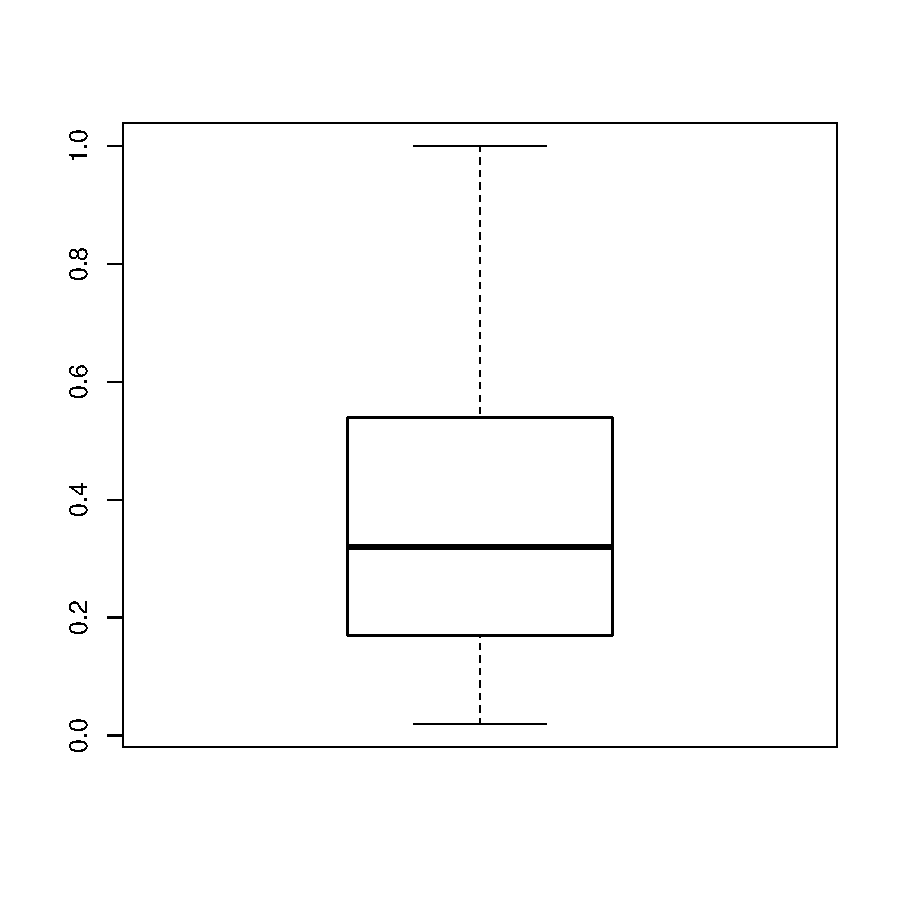
\includegraphics{week1-018}
\begin{Schunk}
\begin{Sinput}
> numericresp <- as.numeric(unlist(response))
> hist(numericresp, xlab ="Crime Rate", main="Histogram of Reported Crime Rate")
\end{Sinput}
\end{Schunk}
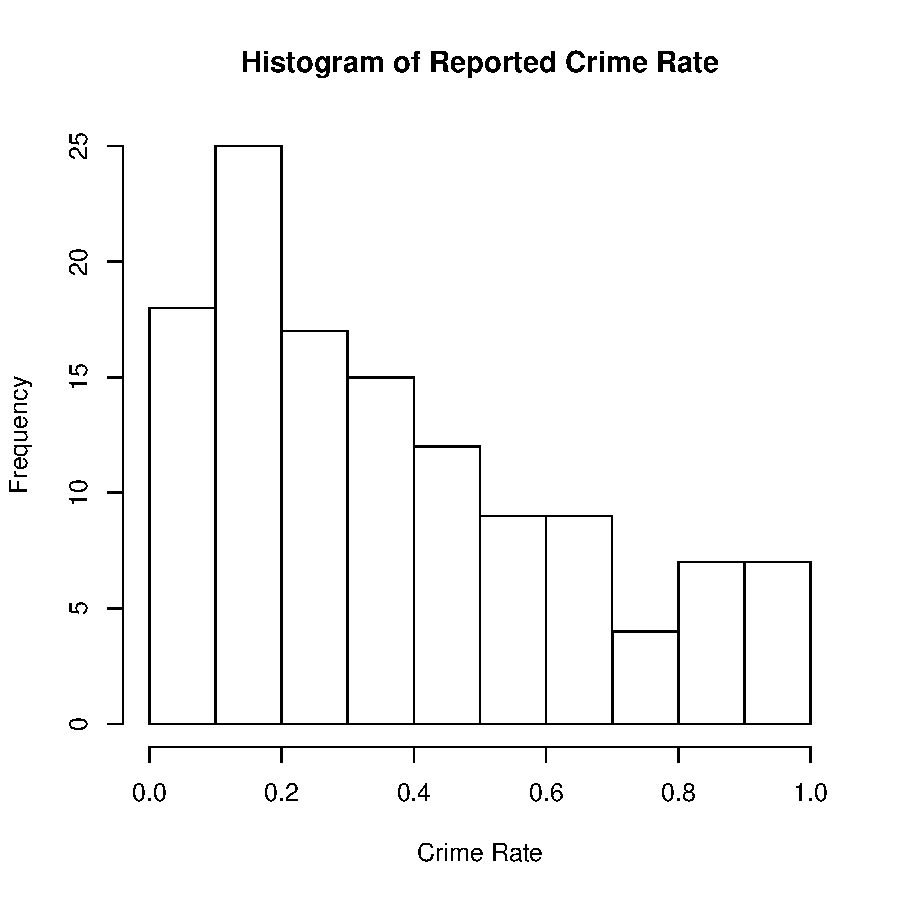
\includegraphics{week1-019}
\begin{Schunk}
\begin{Sinput}
> dfnumeric <- subset(df, select= -c(communityname))
\end{Sinput}
\end{Schunk}

\end{solution}
\item Identify the top 9 most predictive variable with respect to response (remove instances
with missing values and/or categorical variables if necessary)
\begin{solution}
We generate a loop over the above data frame and create a correlation vector with respect to response
\begin{Schunk}
\begin{Sinput}
> correlationVector <- c()
> for(i in 1:ncol(dfnumeric)) {
+   correlationVector <- c(correlationVector, cor(dfnumeric[,i], response))
+ }
> names(correlationVector) <- colnames(dfnumeric)
> #correlationVector 
> sortnames <- name[,2][order(abs(correlationVector), decreasing = TRUE)[1:9]]
> sortnames
\end{Sinput}
\begin{Soutput}
[1] PolicBudgPerPop  PctFam2Par       PersPerFam       PctYoungKids2Par
[5] NumIlleg         PctKids2Par      racepctblack     pctWSocSec      
[9] pctWFarmSelf    
128 Levels: agePct12t21 agePct12t29 agePct16t24 agePct65up ... whitePerCap
\end{Soutput}
\end{Schunk}
\end{solution}
\item Generate histogram, estimate density, and boxplot for each of these predictive
variables 
\begin{solution}
We generate a new dataframe composed of the 9 highly correlated variables:
\begin{Schunk}
\begin{Sinput}
> df9 <- subset(dfnumeric, select = c("PolicBudgPerPop", "PctFam2Par", "PersPerFam", "PctYoungKids2Par", "NumIlleg", "PctKids2Par", "racepctblack", "pctWSocSec","pctWFarmSelf"))
> par(mfrow = c(3, 3))
> for (i in names(df9)) {
+   x <- df9[,i]
+   hist(x, main = i)
+ }
> 
\end{Sinput}
\end{Schunk}
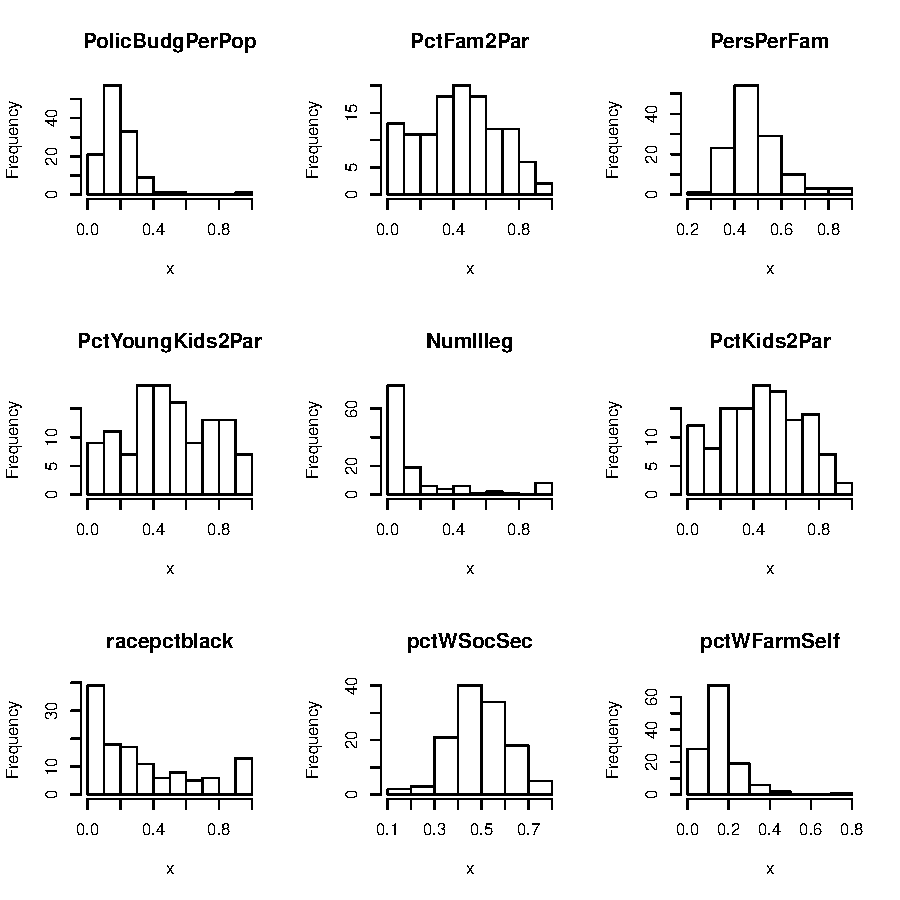
\includegraphics{week1-022}
\begin{Schunk}
\begin{Sinput}
> par(mfrow = c(3, 3))
> for (i in names(df9)) {
+   x <- df9[,i]
+   boxplot(x, main = i)
+   
+ }
\end{Sinput}
\end{Schunk}
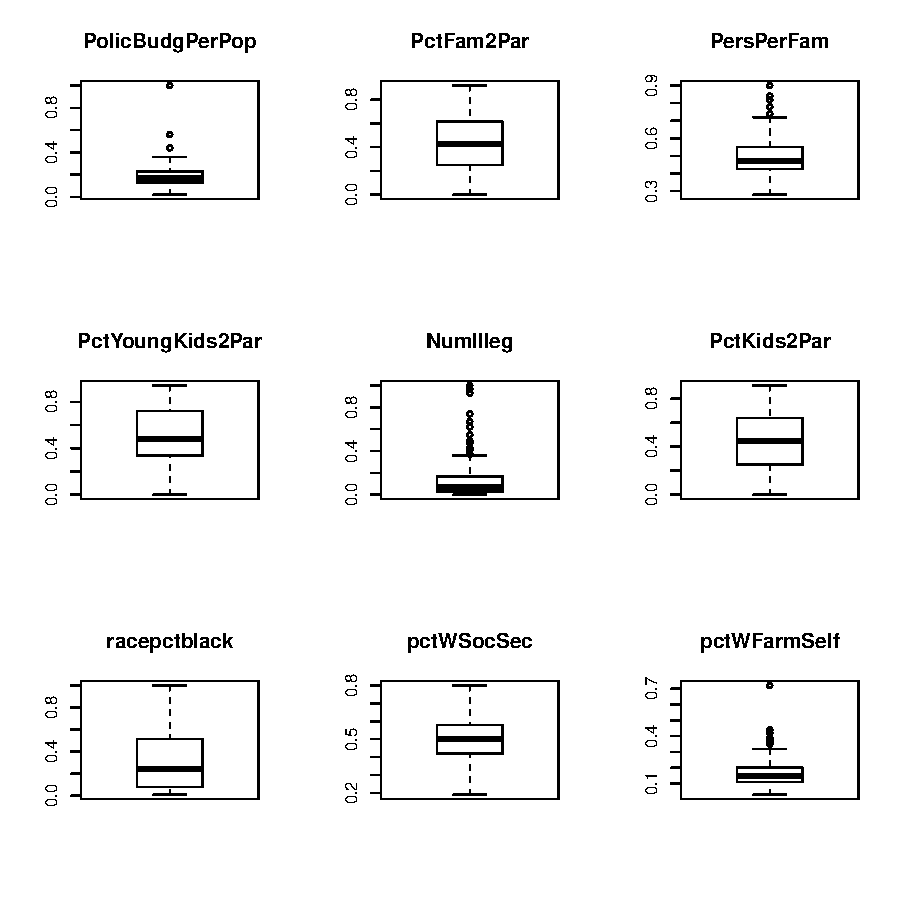
\includegraphics{week1-023}
\begin{Schunk}
\begin{Sinput}
> par(mfrow = c(3, 3))
> for (i in names(df9)) {
+   x <- density(df9[,i])
+   plot(x, main = i) 
+   
+ }
\end{Sinput}
\end{Schunk}
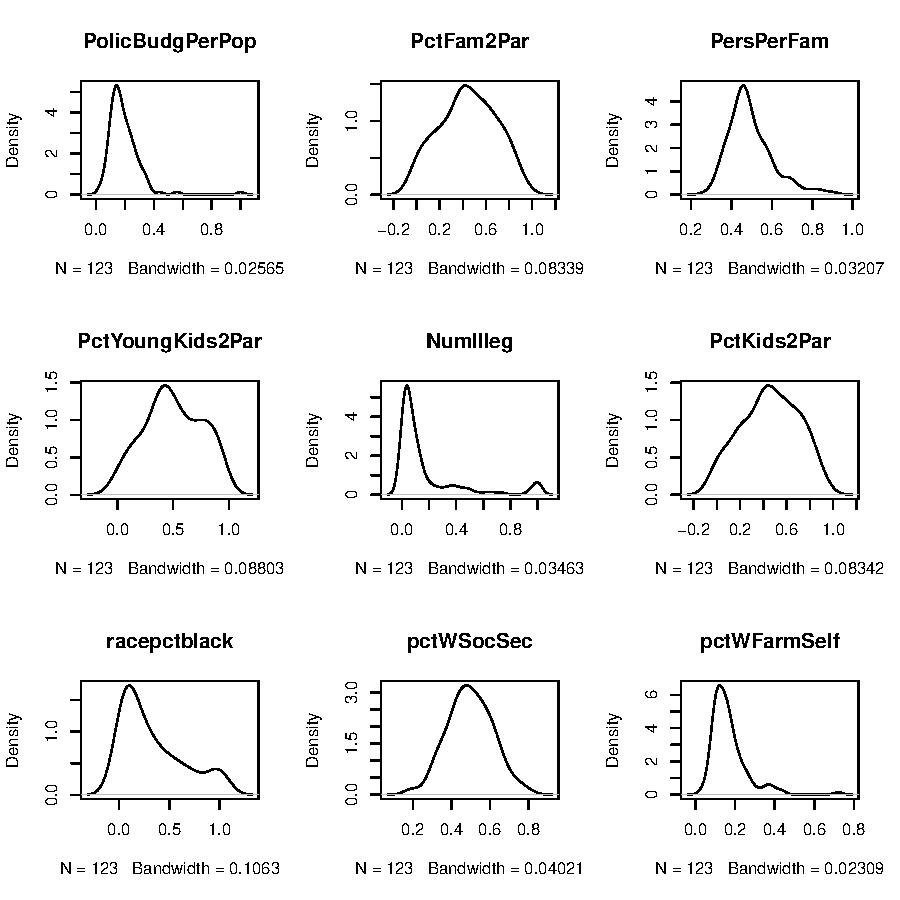
\includegraphics{week1-024}

\end{solution}
\item Are these highly predictive variables correlated with each other?
\begin{solution}
\begin{Schunk}
\begin{Sinput}
> res <- cor(df9)
> round(res, 2)
\end{Sinput}
\begin{Soutput}
                 PolicBudgPerPop PctFam2Par PersPerFam PctYoungKids2Par
PolicBudgPerPop             1.00      -0.32       0.07            -0.23
PctFam2Par                 -0.32       1.00      -0.34             0.97
PersPerFam                  0.07      -0.34       1.00            -0.35
PctYoungKids2Par           -0.23       0.97      -0.35             1.00
NumIlleg                    0.27      -0.65       0.29            -0.63
PctKids2Par                -0.31       0.99      -0.39             0.96
racepctblack                0.31      -0.75       0.44            -0.68
pctWSocSec                 -0.11       0.07      -0.15             0.05
pctWFarmSelf               -0.11       0.37      -0.29             0.35
                 NumIlleg PctKids2Par racepctblack pctWSocSec pctWFarmSelf
PolicBudgPerPop      0.27       -0.31         0.31      -0.11        -0.11
PctFam2Par          -0.65        0.99        -0.75       0.07         0.37
PersPerFam           0.29       -0.39         0.44      -0.15        -0.29
PctYoungKids2Par    -0.63        0.96        -0.68       0.05         0.35
NumIlleg             1.00       -0.65         0.67      -0.14        -0.23
PctKids2Par         -0.65        1.00        -0.78       0.09         0.38
racepctblack         0.67       -0.78         1.00      -0.20        -0.33
pctWSocSec          -0.14        0.09        -0.20       1.00        -0.25
pctWFarmSelf        -0.23        0.38        -0.33      -0.25         1.00
\end{Soutput}
\begin{Sinput}
> heatmap(res)
\end{Sinput}
\end{Schunk}
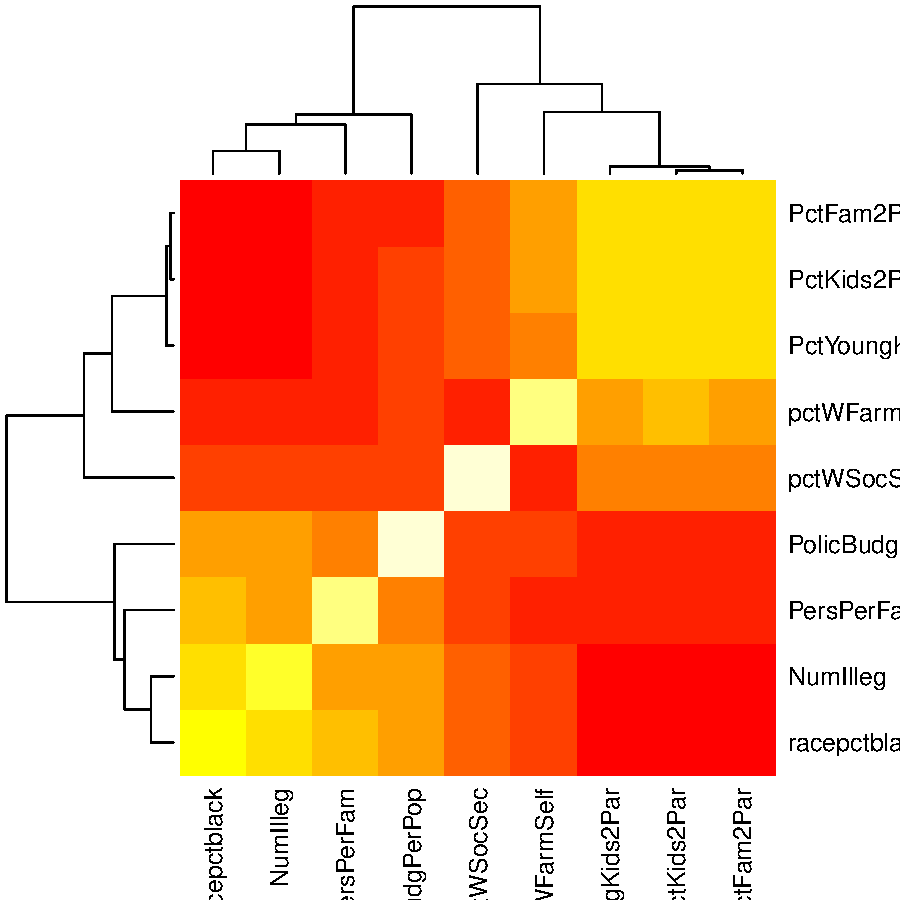
\includegraphics{week1-025}

\end{solution}
\end{enumerate}

\end{document}
